% Options for packages loaded elsewhere
\PassOptionsToPackage{unicode}{hyperref}
\PassOptionsToPackage{hyphens}{url}
%
\documentclass[
]{article}
\usepackage{lmodern}
\usepackage{amssymb,amsmath}
\usepackage{ifxetex,ifluatex}
\ifnum 0\ifxetex 1\fi\ifluatex 1\fi=0 % if pdftex
  \usepackage[T1]{fontenc}
  \usepackage[utf8]{inputenc}
  \usepackage{textcomp} % provide euro and other symbols
\else % if luatex or xetex
  \usepackage{unicode-math}
  \defaultfontfeatures{Scale=MatchLowercase}
  \defaultfontfeatures[\rmfamily]{Ligatures=TeX,Scale=1}
\fi
% Use upquote if available, for straight quotes in verbatim environments
\IfFileExists{upquote.sty}{\usepackage{upquote}}{}
\IfFileExists{microtype.sty}{% use microtype if available
  \usepackage[]{microtype}
  \UseMicrotypeSet[protrusion]{basicmath} % disable protrusion for tt fonts
}{}
\makeatletter
\@ifundefined{KOMAClassName}{% if non-KOMA class
  \IfFileExists{parskip.sty}{%
    \usepackage{parskip}
  }{% else
    \setlength{\parindent}{0pt}
    \setlength{\parskip}{6pt plus 2pt minus 1pt}}
}{% if KOMA class
  \KOMAoptions{parskip=half}}
\makeatother
\usepackage{xcolor}
\IfFileExists{xurl.sty}{\usepackage{xurl}}{} % add URL line breaks if available
\IfFileExists{bookmark.sty}{\usepackage{bookmark}}{\usepackage{hyperref}}
\hypersetup{
  pdftitle={Assignments},
  hidelinks,
  pdfcreator={LaTeX via pandoc}}
\urlstyle{same} % disable monospaced font for URLs
\usepackage[margin=1in]{geometry}
\usepackage{color}
\usepackage{fancyvrb}
\newcommand{\VerbBar}{|}
\newcommand{\VERB}{\Verb[commandchars=\\\{\}]}
\DefineVerbatimEnvironment{Highlighting}{Verbatim}{commandchars=\\\{\}}
% Add ',fontsize=\small' for more characters per line
\usepackage{framed}
\definecolor{shadecolor}{RGB}{248,248,248}
\newenvironment{Shaded}{\begin{snugshade}}{\end{snugshade}}
\newcommand{\AlertTok}[1]{\textcolor[rgb]{0.94,0.16,0.16}{#1}}
\newcommand{\AnnotationTok}[1]{\textcolor[rgb]{0.56,0.35,0.01}{\textbf{\textit{#1}}}}
\newcommand{\AttributeTok}[1]{\textcolor[rgb]{0.77,0.63,0.00}{#1}}
\newcommand{\BaseNTok}[1]{\textcolor[rgb]{0.00,0.00,0.81}{#1}}
\newcommand{\BuiltInTok}[1]{#1}
\newcommand{\CharTok}[1]{\textcolor[rgb]{0.31,0.60,0.02}{#1}}
\newcommand{\CommentTok}[1]{\textcolor[rgb]{0.56,0.35,0.01}{\textit{#1}}}
\newcommand{\CommentVarTok}[1]{\textcolor[rgb]{0.56,0.35,0.01}{\textbf{\textit{#1}}}}
\newcommand{\ConstantTok}[1]{\textcolor[rgb]{0.00,0.00,0.00}{#1}}
\newcommand{\ControlFlowTok}[1]{\textcolor[rgb]{0.13,0.29,0.53}{\textbf{#1}}}
\newcommand{\DataTypeTok}[1]{\textcolor[rgb]{0.13,0.29,0.53}{#1}}
\newcommand{\DecValTok}[1]{\textcolor[rgb]{0.00,0.00,0.81}{#1}}
\newcommand{\DocumentationTok}[1]{\textcolor[rgb]{0.56,0.35,0.01}{\textbf{\textit{#1}}}}
\newcommand{\ErrorTok}[1]{\textcolor[rgb]{0.64,0.00,0.00}{\textbf{#1}}}
\newcommand{\ExtensionTok}[1]{#1}
\newcommand{\FloatTok}[1]{\textcolor[rgb]{0.00,0.00,0.81}{#1}}
\newcommand{\FunctionTok}[1]{\textcolor[rgb]{0.00,0.00,0.00}{#1}}
\newcommand{\ImportTok}[1]{#1}
\newcommand{\InformationTok}[1]{\textcolor[rgb]{0.56,0.35,0.01}{\textbf{\textit{#1}}}}
\newcommand{\KeywordTok}[1]{\textcolor[rgb]{0.13,0.29,0.53}{\textbf{#1}}}
\newcommand{\NormalTok}[1]{#1}
\newcommand{\OperatorTok}[1]{\textcolor[rgb]{0.81,0.36,0.00}{\textbf{#1}}}
\newcommand{\OtherTok}[1]{\textcolor[rgb]{0.56,0.35,0.01}{#1}}
\newcommand{\PreprocessorTok}[1]{\textcolor[rgb]{0.56,0.35,0.01}{\textit{#1}}}
\newcommand{\RegionMarkerTok}[1]{#1}
\newcommand{\SpecialCharTok}[1]{\textcolor[rgb]{0.00,0.00,0.00}{#1}}
\newcommand{\SpecialStringTok}[1]{\textcolor[rgb]{0.31,0.60,0.02}{#1}}
\newcommand{\StringTok}[1]{\textcolor[rgb]{0.31,0.60,0.02}{#1}}
\newcommand{\VariableTok}[1]{\textcolor[rgb]{0.00,0.00,0.00}{#1}}
\newcommand{\VerbatimStringTok}[1]{\textcolor[rgb]{0.31,0.60,0.02}{#1}}
\newcommand{\WarningTok}[1]{\textcolor[rgb]{0.56,0.35,0.01}{\textbf{\textit{#1}}}}
\usepackage{graphicx,grffile}
\makeatletter
\def\maxwidth{\ifdim\Gin@nat@width>\linewidth\linewidth\else\Gin@nat@width\fi}
\def\maxheight{\ifdim\Gin@nat@height>\textheight\textheight\else\Gin@nat@height\fi}
\makeatother
% Scale images if necessary, so that they will not overflow the page
% margins by default, and it is still possible to overwrite the defaults
% using explicit options in \includegraphics[width, height, ...]{}
\setkeys{Gin}{width=\maxwidth,height=\maxheight,keepaspectratio}
% Set default figure placement to htbp
\makeatletter
\def\fps@figure{htbp}
\makeatother
\setlength{\emergencystretch}{3em} % prevent overfull lines
\providecommand{\tightlist}{%
  \setlength{\itemsep}{0pt}\setlength{\parskip}{0pt}}
\setcounter{secnumdepth}{-\maxdimen} % remove section numbering

\title{Assignments}
\author{}
\date{\vspace{-2.5em}}

\begin{document}
\maketitle

{
\setcounter{tocdepth}{1}
\tableofcontents
}
\hypertarget{assignment-1}{%
\section{Assignment 1}\label{assignment-1}}

\textbf{Collaborators: Carolina Herrera Figueroa. }

\hypertarget{problem-1}{%
\subsubsection{Problem 1}\label{problem-1}}

Install the datasets package on the console below and load the data

\begin{Shaded}
\begin{Highlighting}[]
\NormalTok{dat<-USArrests}
\end{Highlighting}
\end{Shaded}

Load the USArrests dataset and rename it \texttt{dat}. Note that this
dataset comes with R, in the package datasets, so there's no need to
load data from your computer. Why is it useful to rename the dataset?

Answer: It is useful to rename the data set for convenience and easy
accessibility.

\begin{Shaded}
\begin{Highlighting}[]
\NormalTok{USArrests}
\end{Highlighting}
\end{Shaded}

\begin{verbatim}
##                Murder Assault UrbanPop Rape
## Alabama          13.2     236       58 21.2
## Alaska           10.0     263       48 44.5
## Arizona           8.1     294       80 31.0
## Arkansas          8.8     190       50 19.5
## California        9.0     276       91 40.6
## Colorado          7.9     204       78 38.7
## Connecticut       3.3     110       77 11.1
## Delaware          5.9     238       72 15.8
## Florida          15.4     335       80 31.9
## Georgia          17.4     211       60 25.8
## Hawaii            5.3      46       83 20.2
## Idaho             2.6     120       54 14.2
## Illinois         10.4     249       83 24.0
## Indiana           7.2     113       65 21.0
## Iowa              2.2      56       57 11.3
## Kansas            6.0     115       66 18.0
## Kentucky          9.7     109       52 16.3
## Louisiana        15.4     249       66 22.2
## Maine             2.1      83       51  7.8
## Maryland         11.3     300       67 27.8
## Massachusetts     4.4     149       85 16.3
## Michigan         12.1     255       74 35.1
## Minnesota         2.7      72       66 14.9
## Mississippi      16.1     259       44 17.1
## Missouri          9.0     178       70 28.2
## Montana           6.0     109       53 16.4
## Nebraska          4.3     102       62 16.5
## Nevada           12.2     252       81 46.0
## New Hampshire     2.1      57       56  9.5
## New Jersey        7.4     159       89 18.8
## New Mexico       11.4     285       70 32.1
## New York         11.1     254       86 26.1
## North Carolina   13.0     337       45 16.1
## North Dakota      0.8      45       44  7.3
## Ohio              7.3     120       75 21.4
## Oklahoma          6.6     151       68 20.0
## Oregon            4.9     159       67 29.3
## Pennsylvania      6.3     106       72 14.9
## Rhode Island      3.4     174       87  8.3
## South Carolina   14.4     279       48 22.5
## South Dakota      3.8      86       45 12.8
## Tennessee        13.2     188       59 26.9
## Texas            12.7     201       80 25.5
## Utah              3.2     120       80 22.9
## Vermont           2.2      48       32 11.2
## Virginia          8.5     156       63 20.7
## Washington        4.0     145       73 26.2
## West Virginia     5.7      81       39  9.3
## Wisconsin         2.6      53       66 10.8
## Wyoming           6.8     161       60 15.6
\end{verbatim}

\begin{Shaded}
\begin{Highlighting}[]
\NormalTok{dat<-USArrests}
\end{Highlighting}
\end{Shaded}

\hypertarget{problem-2}{%
\subsubsection{Problem 2}\label{problem-2}}

List the variables contained in the dataset:

The four variables within the dataset are Murder, Assault, Urbanpop and
Rape

\hypertarget{problem-3}{%
\subsubsection{Problem 3}\label{problem-3}}

What type of variable (from the DVB chapter) is \texttt{Murder}?

Answer: categorical

What R Type of variable is it?

Answer: character

\hypertarget{problem-4}{%
\subsubsection{Problem 4}\label{problem-4}}

What information is contained in this dataset, in general? What do the
numbers mean?

Answer: The data set shows the arrest rate per 100,000 in the US in
1973. The rows show each state and the columns show the type of arrest.
Each number shows the amount of arrests of that type within that state.

\hypertarget{problem-5}{%
\subsubsection{Problem 5}\label{problem-5}}

Draw a histogram of \texttt{Murder} with proper labels and title.

I chose to do a bar chart instead due to the categorical nature of the
values.

\begin{Shaded}
\begin{Highlighting}[]
\NormalTok{  state.names =}\StringTok{ }\KeywordTok{row.names}\NormalTok{(USArrests)}
\KeywordTok{barplot}\NormalTok{(USArrests}\OperatorTok{$}\NormalTok{Murder, }\DataTypeTok{names.arg =}\NormalTok{ state.names, }\DataTypeTok{las =} \DecValTok{2}\NormalTok{, }\DataTypeTok{ylab =} \StringTok{"Arrest rate for Murder per 100,000"}\NormalTok{, }
    \DataTypeTok{main =} \StringTok{"Arrest rate for Murder in the United States in 1973"}\NormalTok{)}
\end{Highlighting}
\end{Shaded}

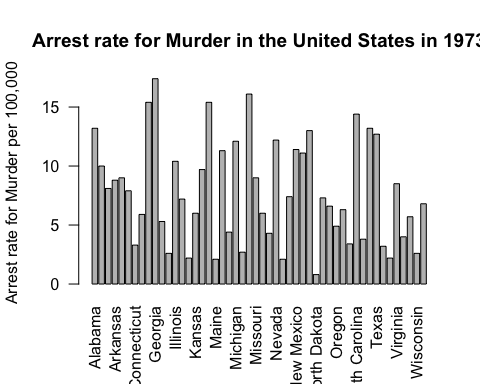
\includegraphics{Assignments_files/figure-latex/unnamed-chunk-3-1.pdf}

\hypertarget{problem-6}{%
\subsubsection{Problem 6}\label{problem-6}}

Please summarize \texttt{Murder} quantitatively. What are its mean and
median? What is the difference between mean and median? What is a
quartile, and why do you think R gives you the 1st Qu. and 3rd Qu.?

Answer: The mean for murder is 7.888 and the mean for murder is 7.250.
Mean is the average of the data (that is: if you were to add up all of
the values then divide by the amount of values present). Median is the
middle value (half of the values are above and half are below). If the
data is well distributed, mean and median will be similar or the same,
but the major differences occur when there are outliers: mean is
impacted by outliers whereas median is not. In this data seet, mean and
median appear rather similar. Quartiles are the data broken up into 4
parts. R gives the 1st quartile to give a sense of the values up until
25\% of the data and the 3rd quartile to give values up until 75\% of
the data.

\hypertarget{problem-7}{%
\subsubsection{Problem 7}\label{problem-7}}

Repeat the same steps you followed for \texttt{Murder}, for the
variables \texttt{Assault} and \texttt{Rape}. Now plot all three
histograms together. You can do this by using the command
\texttt{par(mfrow=c(3,1))} and then plotting each of the three.

\begin{Shaded}
\begin{Highlighting}[]
\NormalTok{  state.names =}\StringTok{ }\KeywordTok{row.names}\NormalTok{(USArrests)}
\KeywordTok{barplot}\NormalTok{(USArrests}\OperatorTok{$}\NormalTok{Assault, }\DataTypeTok{names.arg =}\NormalTok{ state.names, }\DataTypeTok{las =} \DecValTok{2}\NormalTok{, }\DataTypeTok{ylab =} \StringTok{"Arrest rate for assault per 100,000"}\NormalTok{, }
    \DataTypeTok{main =} \StringTok{"Arrest Rate for Assault in the United States in 1973"}\NormalTok{)}
\end{Highlighting}
\end{Shaded}

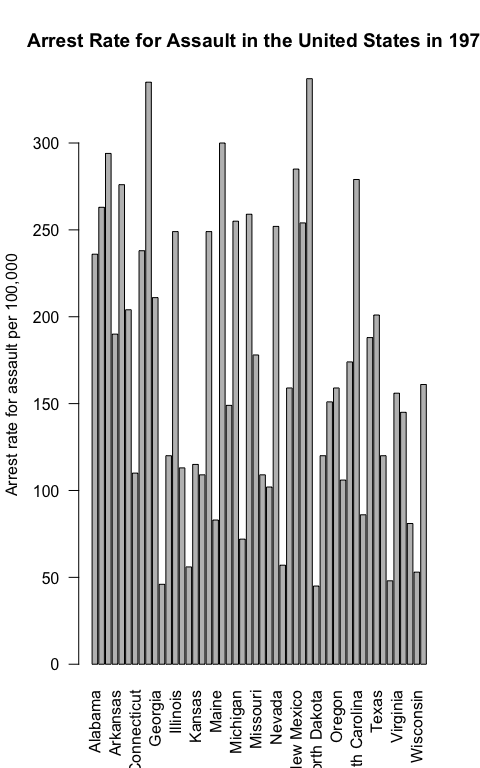
\includegraphics{Assignments_files/figure-latex/unnamed-chunk-4-1.pdf}

\begin{Shaded}
\begin{Highlighting}[]
\NormalTok{ state.names =}\StringTok{ }\KeywordTok{row.names}\NormalTok{(USArrests)}
\KeywordTok{barplot}\NormalTok{(USArrests}\OperatorTok{$}\NormalTok{Rape, }\DataTypeTok{names.arg =}\NormalTok{ state.names, }\DataTypeTok{las =} \DecValTok{2}\NormalTok{, }\DataTypeTok{ylab =} \StringTok{"Arrest rate for Rape per 100,000"}\NormalTok{, }
    \DataTypeTok{main =} \StringTok{"Arrest Rate for Rape in the United States in 1973"}\NormalTok{)}
\end{Highlighting}
\end{Shaded}

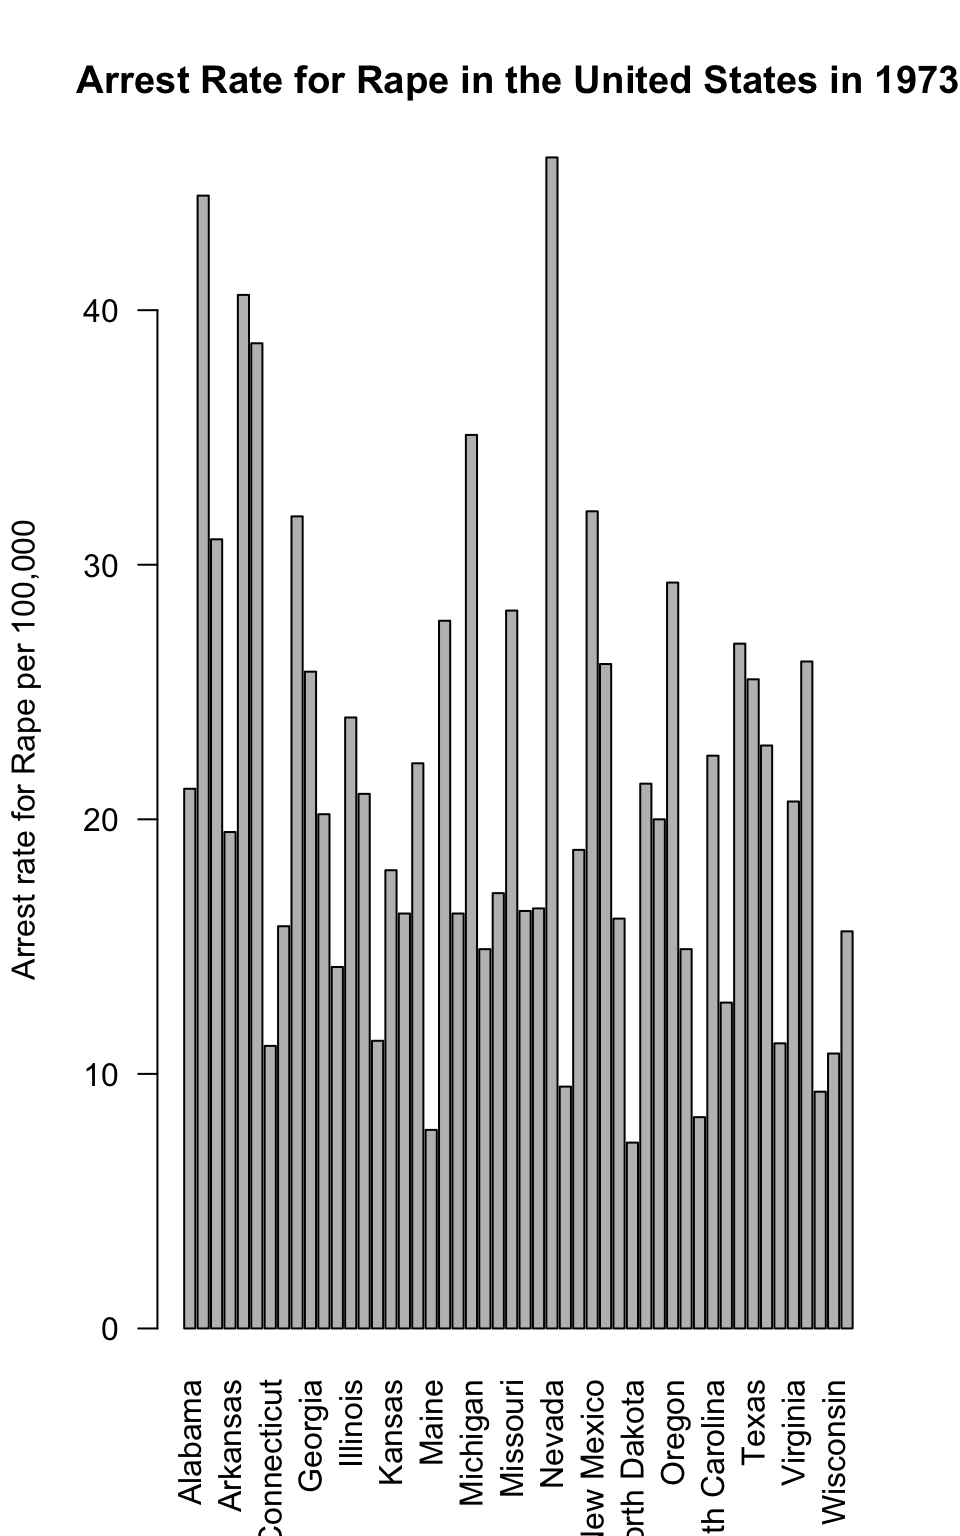
\includegraphics{Assignments_files/figure-latex/unnamed-chunk-4-2.pdf}

\begin{Shaded}
\begin{Highlighting}[]
   \KeywordTok{par}\NormalTok{(}\DataTypeTok{mfrow=}\KeywordTok{c}\NormalTok{(}\DecValTok{3}\NormalTok{,}\DecValTok{1}\NormalTok{))}
\NormalTok{     state.names =}\StringTok{ }\KeywordTok{row.names}\NormalTok{(USArrests)}
\KeywordTok{barplot}\NormalTok{(USArrests}\OperatorTok{$}\NormalTok{Murder, }\DataTypeTok{names.arg =}\NormalTok{ state.names, }\DataTypeTok{las =} \DecValTok{2}\NormalTok{, }\DataTypeTok{ylab =} \StringTok{"Arrest rate for Murder per 100,000"}\NormalTok{, }
    \DataTypeTok{main =} \StringTok{"Arrest rate for Murder in the United States in 1973"}\NormalTok{)}

\NormalTok{state.names =}\StringTok{ }\KeywordTok{row.names}\NormalTok{(USArrests)}
\KeywordTok{barplot}\NormalTok{(USArrests}\OperatorTok{$}\NormalTok{Assault, }\DataTypeTok{names.arg =}\NormalTok{ state.names, }\DataTypeTok{las =} \DecValTok{2}\NormalTok{, }\DataTypeTok{ylab =} \StringTok{"Arrest rate for assault per 100,000"}\NormalTok{, }
    \DataTypeTok{main =} \StringTok{"Arrest Rate for Assault in the United States in 1973"}\NormalTok{)}

\NormalTok{ state.names =}\StringTok{ }\KeywordTok{row.names}\NormalTok{(USArrests)}
\KeywordTok{barplot}\NormalTok{(USArrests}\OperatorTok{$}\NormalTok{Rape, }\DataTypeTok{names.arg =}\NormalTok{ state.names, }\DataTypeTok{las =} \DecValTok{2}\NormalTok{, }\DataTypeTok{ylab =} \StringTok{"Arrest rate for Rape per 100,000"}\NormalTok{, }
    \DataTypeTok{main =} \StringTok{"Arrest Rate for Rape in the United States in 1973"}\NormalTok{)}
\end{Highlighting}
\end{Shaded}

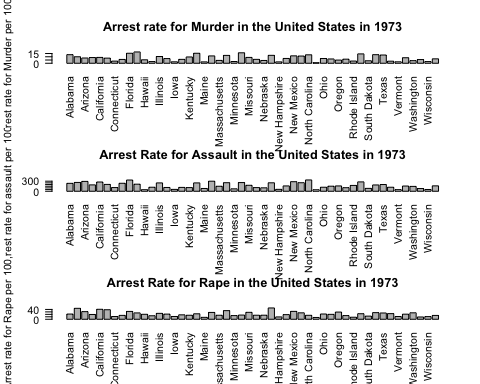
\includegraphics{Assignments_files/figure-latex/unnamed-chunk-5-1.pdf}

What does the command par do, in your own words (you can look this up by
asking R \texttt{?par})?

Answer: Command par allows for multiple graphs to be plotted together.
This command makes this possible by defining parameters.

What can you learn from plotting the histograms together?

Answer: By plotting the histograms together it allows us to visually
compare the rates for each. While it is useful to compare the numbers
when looking at the table, plotting the values together allows for
visual comparison.

\hypertarget{problem-8}{%
\subsubsection{Problem 8}\label{problem-8}}

What does the given code do? Explain what each line is doing.

Answer: This code creates a heat map of murders in the US. That is, this
is a map of the country with darker shades of blue signifying higher
murder rates and lighter shades of blue portraying lower murder rates.
The first line tells R that you will be making a heat map, arranging by
state and filling with arrests for murder rates. The next line sets up
the map itself separating by state and the final line expands the range

\[\\[2in]\]

\end{document}
